\documentclass[12pt]{book}

\usepackage{amsmath, amsthm, mathtools, amssymb}
\usepackage{thmtools}

\usepackage{enumitem}
\usepackage{parskip}
\usepackage{pdfpages}
\usepackage{float}
\usepackage{tikz}
\usepackage{graphicx}
\usepackage[utf8]{inputenc}
\usepackage{listings}
\usepackage{array}
\usetikzlibrary{automata, arrows.meta, positioning}

\newcommand{\HRule}[1]{\rule{\linewidth}{#1}}

\declaretheoremstyle[name=Theorem,]{thmsty}
\declaretheorem[style=thmsty,numberwithin=section]{theorem}

\declaretheoremstyle[name=Definition,]{prosty}
\declaretheorem[style=prosty,numberlike=theorem]{definition}

\newtheorem{lemma}{Lemma}[section]

\newcommand*{\successor}{%
    \stackrel{\scriptscriptstyle\!+\!}\longrightarrow%
}

\newcommand*{\lsuccessor}{%
    \stackrel{\scriptscriptstyle\!+\!}\longleftarrow%
}

\newcommand*{\too}{%
    \stackrel{\scriptscriptstyle\!*\!}\longrightarrow%
}

\newcommand*{\ltoo}{%
    \stackrel{\scriptscriptstyle\!*\!}\longleftarrow%
}

\makeatletter
\newcommand{\chapterauthor}[1]{%
  {\parindent0pt\vspace*{-25pt}%
  \linespread{1.1}\large\scshape#1%
  \par\nobreak\vspace*{35pt}}
  \@afterheading%
}
\makeatother

\begin{document}

\title{Lecture Notes}
\date{}
\maketitle
\newpage

\tableofcontents

\chapter{Lecture 2}

\subsection{Abstract Reduction System}
An abstract reduction system is a binary relation $\rightarrow$ over a set of elements $A$.

\subsection{Other Relations defined on $\protect\overrightarrow{A}$}
\begin{description}[labelsep=4em, align=left, labelwidth=2in]

\item[Identity] $\overrightarrow{A^0} = \{(a, a): a \in A\}$

\item[Reflexive Closure] $\overrightarrow{A^=} = \overrightarrow{A} \cup \overrightarrow{A^0}$

\item[Inverse] $\overrightarrow{A^{-1}} = \{(b, a): a \xrightarrow[A]{} b\}$

\item[Transitive Closure] $\overrightarrow{A^+} = \bigcup\limits_{i \, > \, 0} \overrightarrow{A^i}$

\item[Reflexive Transitive Closure] $\overrightarrow{A^*} = \overrightarrow{A^+} \cup \overrightarrow{A^0}$

\item[Symmetric closure] $\overrightarrow{A^\leftrightarrow} = \overrightarrow{A} \cup \overrightarrow{A^{-1}}$

\end{description}

\vspace{2em}

\textbf{Note:} Pay attention to the order of terms in the name of the relations. For example, the transitive symmetric closure isn't necessarily the same as the symmetric transitive closure. Consider the following relation graph to demonstrate this.

\vspace{2em}

\begin{figure}[!h]
\centering
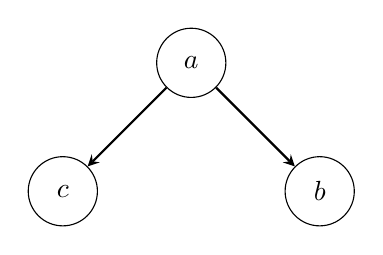
\begin{tikzpicture}
	\node (a) [state] {$a$};
	\node (b) [state, below right = of a] {$b$};
	\node (c) [state, below left = of a] {$c$};
	
	\path [-stealth, thick]
		(a) edge node {} (b)
		(a) edge node {} (c);
		
\end{tikzpicture}
\end{figure}

\begin{align*}
{(A^\leftrightarrow)}^* &= \{(a, a), (a, b), (a, c), (b, a), (b, b), (b, c), (c, a), (c, b), (c, c)\}\\ 
{({A^*})}^\leftrightarrow &= \{(a, b), (a, c), (b, a), (c, a)\}
\end{align*}

\newpage
\subsection{Terminology}

\subsubsection{Describing the elements and their relations}

\begin{itemize}
\item $x$ is reducible if $\exists \, x'$ such that $x \xrightarrow[A]{} x'$.

\item $\theta: F \rightarrow E$ is called an \textbf{invariant} if $\forall x \in A, \theta(x) = \theta(F(x))$. For example, for the run $x_0 \xrightarrow[F]{} x_1 \xrightarrow[F]{} x_2 \xrightarrow[F]{} \cdots$, it must hold that $\theta(x_0) = \theta(x_1) = \theta(x_2) = \cdots$.

\item $x$ is in \textbf{normal form} if it is not reducible.

\item $x$ \textbf{simplifies to} $x'$ in $A$ iff $x \xrightarrow[A^*]{} x'$.

\item $x'$ is a normal form of $x$ in $A$ if: 
\begin{itemize}
\item $x'$ is in normal form
\item $x$ simplifies to $x'$
\end{itemize}

\item $x$ has a normal form in $A$ if $\exists \, x' \in A$ such that $x'$ is a normal form of $x$.

\item $x'$ is an \textbf{immediate successor} of $x$ if $x \xrightarrow[A]{} x'$.

\item $x'$ is a \textbf{proper successor} of $x$ if $x \xrightarrow[A^+]{} x'$.

\item $x'$ is a \textbf{successor} of $x$ if $x \xrightarrow[A^*]{} x'$.

\item Two elements $a$ and $b$ in $A$ are \textbf{joinable} if $\exists \, c \in A$ such that $a \xrightarrow[A^*]{} c$ and $b \xrightarrow[A^*]{} c$. This is denoted as $a \downarrow b$.

\item $a$ and $b$ are \textbf{connected} in $A$ if $a \xrightarrow[{(A^\leftrightarrow)}^*]{} b$

\end{itemize}

\subsubsection{Describing the system as a whole}

\begin{itemize}

\item $\overrightarrow{A}$ is terminating if there is no infinite run: $a_0 \rightarrow a_1 \rightarrow \cdots$.

\begin{figure}[htbp]
\centering
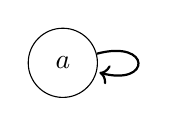
\begin{tikzpicture}
	\node (a) [state] {$a$};
	
	\path [-stealth, thick]
		(a) edge [loop right] node {} (a);
		
\end{tikzpicture}
\caption{A non-terminating relation graph}
\end{figure}

\item $\overrightarrow{A}$ is normalising if every element has a normal form.

\begin{figure}[htbp]
\centering
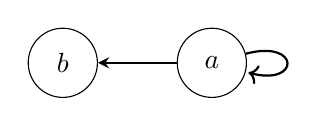
\begin{tikzpicture}
	\node (a) [state] {$a$};
	\node (b) [state, left = of a] {$b$};
	
	\path [-stealth, thick]
		(a) edge [loop right] node {} (a)
		(a) edge node {} (b);
		
\end{tikzpicture}
\caption{A normalising, non-terminating relation graph}
\end{figure}

\item $\overrightarrow{A}$ is confluent if $\forall a, b, c \in A$ such that $a \xrightarrow[A^*]{} b, a \xrightarrow[A^*]{} c$, it must hold that $b \downarrow c$.

\begin{figure}[htbp]
\centering
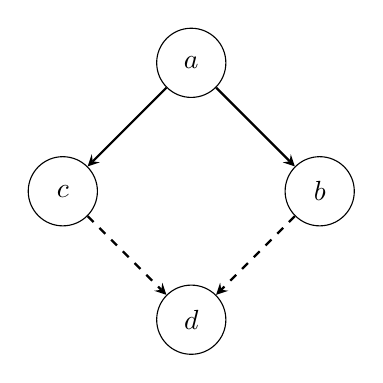
\begin{tikzpicture}
	\node (a) [state] {$a$};
	\node (b) [state, below right = of a] {$b$};
	\node (c) [state, below left = of a] {$c$};
	\node (d) [state, below right = of c] {$d$};
	
	\path [-stealth, thick]
		(a) edge node {} (b)
		(a) edge node {} (c)
		(b) edge [dashed] node {} (d)
		(c) edge [dashed] node {} (d);
		
\end{tikzpicture}
\caption{A visual representation of confluence}
\end{figure}

\end{itemize}

\chapter{Lecture 3}
\chapterauthor{Dheeraja Rajreddygari}

\subsection{Properties of abstract reduction systems}

In this lecture, we explore some properties of abstract reduction systems and look at the relationships between them.

\begin{definition}
    An abstract reduction system $( A, \xrightarrow[A]{} )$ is said to be \textbf{Church-Rosser} if $$\forall x, y \in A, \quad x \xleftrightarrow[A]{*} y \implies x \downarrow_A y$$
\end{definition}

Consider abstract reduction systems $A$ and $B$ as shown in the figure below. System $A$ is not Church-Rosser, since $a \xleftrightarrow[A]{*} b$ but $a$ and $b$ are not joinable. System $B$ is a simple example of a Church-Rosser system.

\begin{figure}[htbp]
    \center
    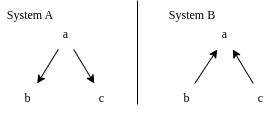
\includegraphics[scale=0.8]{images/lecture1/CR.png}
    \caption{Examples of abstract reduction systems}
\end{figure}


\begin{definition}
    An abstract reduction system $( A, \xrightarrow[A]{} )$ is said to be \textbf{Confluent} if $$\forall a, b, c \in A, \quad a \xrightarrow[A]{*} b \text{ and }  a \xrightarrow[A]{*} c \implies b \downarrow_A c$$
\end{definition}

\begin{definition}
    An abstract reduction system $( A, \xrightarrow[A]{} )$ is said to be \textbf{Semi-confluent} if $$\forall a, b, c \in A, \quad a \xrightarrow[A]{} b \text{ and }  a \xrightarrow[A]{*} c \implies b \downarrow_A c$$
\end{definition}

\begin{theorem}
    For an abstract reduction system, \textbf{Church-Rosser, Confluence and Semi-confluence are equivalent}.
\end{theorem}

\textbf{Proof:} We will prove this theorem in the following three stages. Clearly, the three of them combined result in the theorem stated above.
\begin{enumerate}
    \item $\text{Church-Rosser} \implies \text{Confluence}$
    \item $\text{Confluence} \implies \text{Semi-confluence}$
    \item $\text{Semi-confluence} \implies \text{Church-Rosser}$
\end{enumerate}

First, we will prove that \textbf{if a system is Church-Rosser, it is confluent}. Let $(A, \xrightarrow[A]{})$ be an abstract reduction system that is Church-Rosser. \\
Let $a, b, c \in A : a \xrightarrow[A]{*} b \text{ and } a \xrightarrow[A]{*} c$ \\
By definition, $b \xleftrightarrow[A]{*} c$ \\
Since A is Church-Rosser, $b \xleftrightarrow[A]{*} c \implies b \downarrow_A c$ \\
i.e. $ a \xrightarrow[A]{*} b \text{ and } a \xrightarrow[A]{*} c \implies b \downarrow_A c$, proving that A is confluent


Next, we will prove that \textbf{if a system is Confluent, it is also semi-confluent}. Let $(A, \xrightarrow[A]{})$ be a confluent abstract reduction system. \\
Let $a, b, c \in A : a \xrightarrow[A]{} b \text{ and } a \xrightarrow[A]{*} c$ \\
Since $A \subseteq A^*$, $a \xrightarrow[A]{} b \implies a \xrightarrow[A]{*} b$ \\
Since A is confluent, $a \xrightarrow[A]{*} b \text{ and } a \xrightarrow[A]{*} c \implies b \downarrow_A c$ \\
i.e. $ a \xrightarrow[A]{} b \text{ and } a \xrightarrow[A]{*} c \implies b \downarrow_A c$, proving that A is semi-confluent

Finally, we will prove that \textbf{if a system is semi-confluent, it is also Church-Rosser}. Let $(A, \xrightarrow[A]{})$ be a semi-confluent abstract reduction system. \\
Let $a, b \in A : a \xleftrightarrow[A]{*} b$ \\
Let $p$ be the shortest path connecting $a$ and $b$ in $A^{\leftrightarrow ^*}$. We will use induction on $|p|$ to prove that $a$ and $b$ are joinable. \\
\textbf{Base case:} For $p=0$, we have $a=b$ which makes them trivially joinable. \\
\textbf{Induction step:} Let it be true that if the shortest path connecting $a$ and $b$ in $A^{\leftrightarrow ^*}$ is $|p|$, then $a$ and $b$ are joinable in $A$. We will prove that this is also true for $|p|+1$.

Let $a, b' \in A$ such that the shortest path connecting them in $A^{\leftrightarrow ^*}$ is of length $|p|+1$. Then, $\exists b \in A :$ the shortest path connecting $a$ and $b$ in $A^{\leftrightarrow ^*}$ is $|p|$ and $b \xleftrightarrow[A]{} b'$. Since our induction hypothesis holds true for $|p|$, $a$ and $b$ are joinable (they both reduce to some $c \in A$).


\begin{figure}[htbp]
    \center
    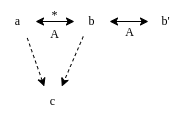
\includegraphics[scale=0.8]{images/lecture1/induction1.png}
    \caption{Abstract reduction system representing the induction step}
\end{figure}
We now have 2 cases. 

\textbf{Case 1:} $b \xleftarrow[A]{} b'$ 

\begin{figure}[htbp]
    \center
    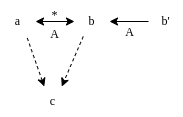
\includegraphics[scale=0.8]{images/lecture1/induction2.png}
    \caption{Abstract reduction system in case 1}
\end{figure}
$b' \xrightarrow[A]{} b \xrightarrow[A]{*} c$. Therefore, $a \downarrow _A b'$. 

\textbf{Case 2:} $b \xrightarrow[A]{} b'$

\begin{figure}[htbp]
    \center
    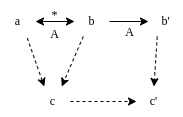
\includegraphics[scale=0.8]{images/lecture1/induction3.png}
    \caption{Abstract reduction system in case 2}
\end{figure}
Here we have $b \xrightarrow[A]{} b'$ and $b \xleftrightarrow[A]{*} c$. Since $A$ is semi-conflient, $b'$ and $c$ must be joinable. That is, $\exists c' \in A : b' \xrightarrow[A]{*} c' \text{ and } c \xrightarrow[A]{*} c'$.  Since $a \xrightarrow[A]{*} c \xrightarrow[A]{*} c'$, we have $a \xrightarrow[A]{*} c'$. Hence, $a \downarrow _A b'$


In either case, we have shown that $a \downarrow _A b'$, which completes our induction. We have proven that $a \xleftrightarrow[A]{*} b \implies a \downarrow_A b$, which means A is also Church-Rosser.

This completes our proof that Church-Rosser, Confluence and Semi-confluence are equivalent properties of an abstract reduction system. While it may seem redundant to have multiple terms to refer to the same thing, they each give us a different perspective of looking at the same property which can prove to be helpful.


\subsection{Address space}
Data structures provide a way to organize and address data. For a data structure, a valid set of addresses form its address space. This is \textbf{not} a formal definition of address spaces and is only meant to give a broad idea. We will look at an example below to illustrate one way of addressing a binary tree. Let us consider the following addressing of a binary tree: each edge is labelled $1$ or $2$ depending on whether it leads to the left or right descendant of a node; the address of each node is obrained by appending the label of the edge leading into it to the address of its parent, with the root being $\epsilon$. Look at the figure below to bettter understand this.
\begin{figure}[htbp]
    \center
    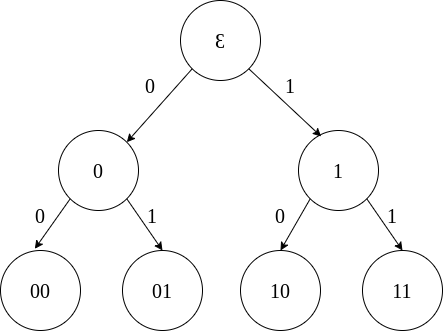
\includegraphics[scale=0.4]{images/lecture1/address.png}
    \caption{Addressing a binary tree}
\end{figure}

The address space for this binary tree would be the set $S = \{\epsilon, 0, 00, 01, 1, 10, 11 \}$. The set $S_1 = \{ \epsilon, 0, 00, 01, 1 \}$ would also be a valid address space for some binary tree but the set $S_2 = \{ 0, 00, 1 \}$ would not, since it does not contain $\epsilon$, the address of the root.

\section{Lecture 4}
\subsection{N-Arity}
$\bar{Z_{n}} = [1...n]$

\subsubsection{}An n-ary address space A is a subset of $\Bar{Z^{*}_{n}}$ that is prefix closed if $q: A$ and $p$ is a prefix of q, then $p: A$.\\

Example:
\begin{figure}[htbp]
    \center
    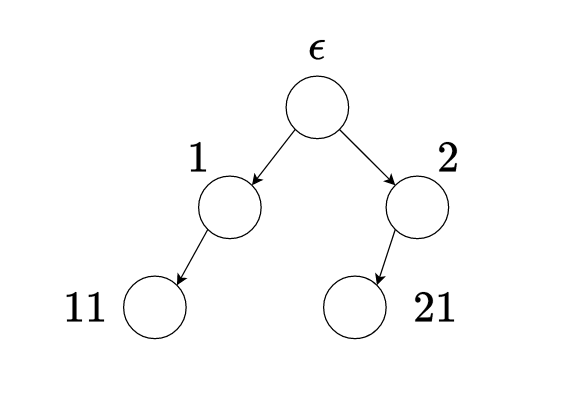
\includegraphics[scale=0.8]{images/popl-4-1.png}
    \caption{}
\end{figure}

$A = {\epsilon, 1, 2, 11, 21}$
\subsubsection{}
Let A be an n-ary address space and let $p:A$ .
\begin{gather}
    A@p = \{q: \bar{Z_{n}^{*}}\  \vert\  pq: A\}  \xrightarrow{} \text{Address space of A relative to p}
\end{gather}

e.g.
\indent $A@2 = \{\epsilon, 1\}$

\subsubsection{}
Context at p (excluding p)
\begin{gather}
    C_{ex}(A, p) = A\backslash pA@p\\
    \xrightarrow{} \text{concatenating p with each address (in subtree) relative to p}
\end{gather}

Context at p (including p)
\begin{gather}
    C_{in}(A, p) = C_{ex}(A,p) \cup \{p\}
\end{gather}
\begin{figure}[htbp]
    \center
    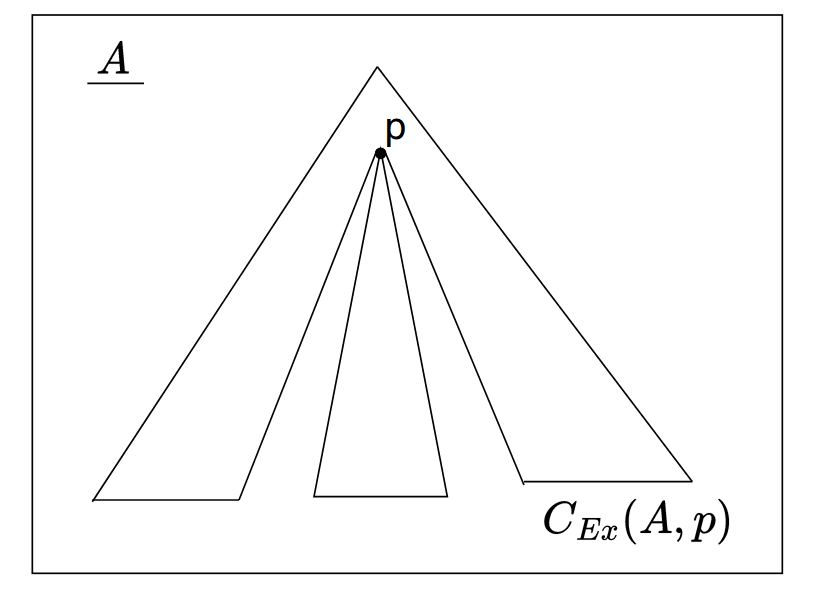
\includegraphics[scale=0.5]{images/popl-4-2.png}
    \caption{}
\end{figure}

\subsection{Terms, Subtrees, Tree Contex}
\subsubsection{}
Let A be an address space. A term is a map $t:A\xrightarrow{}v$ where $V$ is a set of values.

Example:
\begin{gather}
    V = \mathcal{N}, A = \{\epsilon, 1, 2\}\\
    t: \{\epsilon\xrightarrow{}5, 1\xrightarrow{}7, 2\xrightarrow{}7\}
\end{gather}

\begin{figure}[htbp]
    \center
    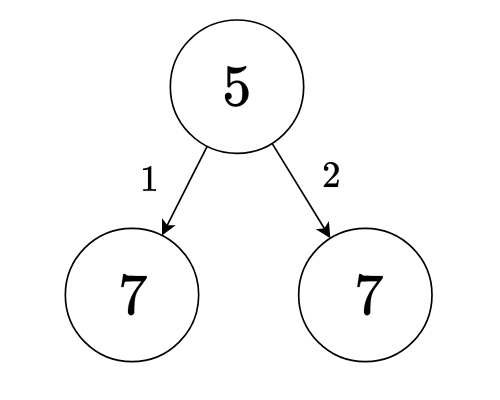
\includegraphics[scale=0.6]{images/popl-4-3.png}
    \caption{}
\end{figure}

\subsubsection{}
Let $t:A\xrightarrow{v}$ be a tree and let $p:A$
\begin{gather}
    C_{ex}(t,p) = df = t \vert_{C_{ex}(A,p}
\end{gather}

\subsubsection{}
Let $\Sigma_{s}$ be a set of symbols.\\
Let $\alpha: \Sigma_{s} \xrightarrow{ \mathcal{N}}$ denote the arity map of $\Sigma_{s}$.\\

Example,\\
\begin{gather}
    \Sigma_{s} = \{f,a,b\}
    \alpha_{s}: \{f\xrightarrow{}2, a\xrightarrow{}0, b\xrightarrow{}0\}\\
    \implies f(a,b) \checkmark \ \ \ \ a \checkmark \ \ \ \ b \checkmark \ \ \ \ f(a) \times
\end{gather}

\subsubsection{}
A term is $(A,\Sigma_{s}, \alpha, t: A\xrightarrow{} \Sigma_{s})$\\
s.t.
\begin{enumerate}
    \item A is a prefix-closed language over $\mathcal{N}_{+}$
    \item $\forall p: A$, if $t_{p}=S$ and $\alpha(S)=n$\\
    then $p1,..., p\alpha(S): A$ \ \ \ \ \  \ \ \ 
    $\forall i: 1 \leq i \leq \alpha(S), pi: A, \forall i: \mathcal{N}_{+}\backslash[1,...,\alpha(S)]pi\notin A$
\end{enumerate}
\newpage

\chapter{Lecture 5}
\chapterauthor{Bharat Sahlot}

\subsection{Terms}

\paragraph{ARS} Abstract Reduction System

\paragraph{Terminating ARS} An ARS is terminating \emph{iff.} it has no infinite runs.

\subsection{Well Founded Induction(WFI)}

This is property of an abstract reduction system. A system having this property implies that,

$$
\forall x \in A. \left( \forall y \in A. \ x \successor y \implies P(y) \right) \implies P(x)
$$

in other words,
$P(x)$ is satisfied if $\forall y. x \successor y \implies P(y)$ is satisfied.

\begin{theorem}
    Let, $(A, \longrightarrow)$ be an ARS, then $A$ satisfies WFI iff. $(A, \longrightarrow)$ is terminating.
\end{theorem}

\begin{proof}
    \text{} \\
    \textbf{1. If $\longrightarrow$ terminates, then $A$ satisfies WFI.} \\
    \emph{Proof by contraposition.} Assume that WFI does not hold. \\
    That implies that $\neg P(a_0)$ for some $a_0 \in A$. Since we assumed that WFI does not hold, $\exists a_1$, such that, $a_0 \successor a_1$ and $\neg P(a_1)$. Using the same arguement, $\exists a_2$, such that, $a_1 \successor a_2$ and $\neg P(a_2)$. Hence there is an infinite chain $a_0 \successor a_1 \successor a_2 \successor ...$, i.e. $\longrightarrow$ does not terminate. \\
    \\
    \textbf{2. If $A$ satisfies WFI, then $\longrightarrow$ terminates.} \\
    \emph{Proof by WFI.} Let,
    $$
    P(x) := \text{there is no infinite chain starting from x}.
    $$
    Clearly, if there is no infinite chain starting from any successor of $x$, then there is no infinite chain starting from $x$. Hence, WFI holds and we can conclude that $P(x)$ holds for all $x$, i.e., $\longrightarrow$ terminates.
\end{proof}

\subsection{Confluence}

Order of evaluation does not matter.

\paragraph{Joinable} $x$ and $y$ are joinable, denoted by $\downarrow$ \emph{iff.} they have the same normal form.

\paragraph{Local Confluence} An element $x \in A$ is said to be locally confluent if $\forall y, z \in A, z \lsuccessor x \successor y$ $\exists w : y \too w \ltoo z$, in other words, $y \downarrow z$.

\paragraph{$\rightarrow$} If a system is terminating and has local confluence for all vertices, then the system has \textbf{confluence}.

\subsection{Interative Evaluation}

\textbf{TODO}

\chapter{Lecture 7}
\chapterauthor{Kommireddy Bhargav Srinivas}
    
    \section{Languages in general}
    
    For any language in general we want to define the following.
    \begin{enumerate}
        \item Define the syntax, which consists of:
            \begin{enumerate}
                \item Abstract syntax (eg: AST)
                \item Concrete Syntax
                \item A Parser, which is a map from concrete syntax to abstract syntax.
                $$
                Parser : Concrete Syntax \rightarrow Abstract Syntax
                $$
            \end{enumerate}
        \item Define the Semantics, which consists of:
            \begin{enumerate}
                \item Semantic domains
                \item An evaluator, which is a map from abstract syntax to the domain of answers.
                $$
                Evaluator : Abstract Syntax \rightarrow Answers 
                $$
            \end{enumerate}
    \end{enumerate}
    
    \begin{figure}[htbp]
        \center
        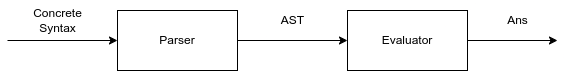
\includegraphics[scale=0.6]{images/lecture7/parser-evaluator.png}
        \caption{Parser Evaluator flow}
    \end{figure}
    
    \subsection{Language 0: ARITHMETIC}
    
    This is a simple language, which works on the integer domain and has the addition, subtraction and multiplication operators defined.
    
    The syntax of the expressions in this language can be defined as follows:
    
    
    \begin{align}
    expr & ::= Num&\\
         & \quad |\quad expr + expr&\\
         & \quad |\quad expr * expr&\\
         & \quad |\quad expr - expr
    \end{align}
    
    where Num represents any Integer.
    Any expression that matches this pattern is a syntactically valid expression in this language.
    
    The semantics of Arithmetic were covered in previous lectures.
    It will consist of the evaluation semantics (eval-ast : AST to Answer)

    The following is the racket implementation of the eval-ast function.
    \lstinputlisting[breaklines]{codes/evalast.rkt}

    \section{Language 1: IF+DIV}

    This language is syntactically a super set of ARITHMETIC. We introduce the if-then-else operator and also division. Division introduces new problems like dividing by zero. We also need to enforce that the condition given to if operator is a boolean.

    These situations cannot be predicted before the program is run for every program. They need to be caught during run-time. In these situations we would like to raise (or throw) errors (or exceptions).

    Now, the result of an expression is not just a number, it could be be a number or an error. There are two ways of dealing with errors, either they are treated specially and the whole execution of the program stops (In racket, you can achieve this using "invoke") and gives the error as the answer to the program. The other way is the treat errors as values, which are returned by the expression that produced the error.

    Errors like non-boolean if-condition (test) or incorrect type being provided to operators (eg: +, -) are called Type Errors
    
    The syntax of the expressions in this language can be defined as follows:
    
    
    \begin{align}
    e & ::= Num&\\
         & \quad |\quad e \quad + \quad e&\\
         & \quad |\quad e \quad * \quad e&\\
         & \quad |\quad e \quad - \quad e&\\
         & \quad |\quad e \quad / \quad e&\\
         & \quad |\quad if \quad e_{test} \quad e_{then} \quad e_{else}
    \end{align}

    The evaluation semantics have an extra rule for division (DIV) similar to addition and multiplication in ARITHMETIC. Along with that we need to define rules to evaluate if-then-else

    $$$$
    $$$$
    
    \begin{displaymath}
             e_{test} \implies \#t, \quad e_{then} \implies v \\
    \end{displaymath}
    % \begin{displaymath}
    \quad\quad\quad\quad\quad\quad\quad
    \textemdash\textemdash\textemdash\textemdash\textemdash\textemdash\textemdash\textemdash\textemdash\textemdash\textemdash\textemdash\textemdash\textemdash\textemdash\textemdash\textemdash\textemdash\textemdash\textemdash IF-TRUE
    % \end{displaymath}

    \begin{displaymath}
        if \quad e_{test} \quad e_{then} \quad e_{else} \implies v
    \end{displaymath}

    $$$$
    \begin{displaymath}
             e_{test} \implies \#f, \quad e_{else} \implies v \\
    \end{displaymath}
    % \begin{displaymath}
    \quad\quad\quad\quad\quad\quad\quad
    \textemdash\textemdash\textemdash\textemdash\textemdash\textemdash\textemdash\textemdash\textemdash\textemdash\textemdash\textemdash\textemdash\textemdash\textemdash\textemdash\textemdash\textemdash\textemdash\textemdash IF-FALSE
    % \end{displaymath}

    \begin{displaymath}
        if \quad e_{test} \quad e_{then} \quad e_{else} \implies v
    \end{displaymath}

    \section{Language-2: GLOBAL}

    A language doesn't need variables (eg: iptables) but programmers do. To make use of variables we need to introduce new constructs called identifiers and environment. Identifiers act as a proxy to values and the environment defines what value a specific identifier takes. (Read later: Combinatory Theory).

    The values that identifiers can take are called denotable values. The values that expressions can take are called expressible values. For the current language both are the same, but languages like C have them different (One cannot store a function in a variable in C).

    The syntax looks almost the same, except the fact that identifiers by themselves are also expressions.

    An environment is a map from identifiers to denotable values.
    
    $$Env: Identifiers \rightarrow Denotable values$$

    In this language, the denotable values is a disjoint union of Numbers and Booleans.

    $$ Denotable values \in Num + Bool $$

    The evaluation semantics change to include the environment as well. 

    \begin{figure}[htbp]
        \center
        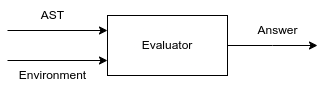
\includegraphics[scale=0.6]{images/lecture7/gloabal-eval.png}
        \caption{Global lang evaluator flow}
    \end{figure}

    When there is a mapping of an identifier in the environment, the identifier is said to be bound to that value. Introduction of identifiers creates a new type of error - Unbound identifier error. This happens when an identifier is used, but it is not bound to any value (It is a free variable.).

    While evaluating the AST if an identifier is encountered, a simple look up is performed in the environment and the corresponding value is taken. The identifier could be bound to an expression. In that case, the expression is evaluated and the corresponding value returned is substituted for the identifier.

    \textbf{Example}
    Expression is ( + x ( * y 2)) and the environment is 
    $$\Gamma = \{ x \mapsto 5, y \mapsto 3, z \mapsto 4\}$$

    We annotate the AST from bottom up get the final value. So we would first annotate x to 5, then y to 3, then get the result of multiplication as 6 and then the result of addition to be 11.

    \begin{figure}[htbp]
        \center
        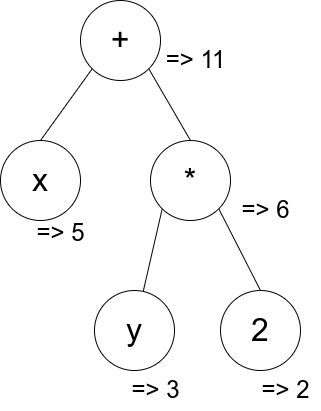
\includegraphics[scale=0.6]{images/lecture7/global_ex_ast.png}
        \caption{Global lang evaluator flow}
    \end{figure}
    
    

\chapter{Lecture 9}
\chapterauthor{Pranav Subramaniam}

% for antecedent-consequent expressions
\newcommand\bigfrac[2]{%
  \begin{array}{c}
    #1 \\
    \hline
    #2
  \end{array}}

\section{Overview of Programming Languages}

\subsection{Mathematical Foundation}
\begin{enumerate}
	\item Before lambda-calculus ("Pre-history" of computing)
	
	\begin{enumerate}
		\item Set Theory
	\end{enumerate}
	\begin{enumerate}
		\item First-Order Logic
	\end{enumerate}
	\begin{enumerate}
		\item Combinatory Logic
	\end{enumerate}
	
	\item Predecessor to Programming Languages \newline
	Provided mathematical framework for programming languages and computing
	
	\begin{enumerate}
		\item Category Theory
		\item $\lambda$ Calculus $\equiv$ Turing Machines (1930s)
		\begin{enumerate}
			\item $\lambda$ Calculus
			\begin{enumerate}
				\item Framework for programming language design
				\item Basis for functional programming
			\end{enumerate}
			\item Turing Machines
			\begin{enumerate}
				\item Computability, complexity, determinism
				\item Related work- Von Neumann architecture, Kurt Gödel's incompleteness theorem
			\end{enumerate}
		\end{enumerate}
	\end{enumerate}
	
\end{enumerate}

\subsection{History}
\begin{table}[H]
  \begin{tabular}{|c|p{2.5cm}|p{2.5cm}|p{2.5cm}|p{2.5cm}|p{2.5cm}|}
    \hline
    \textbf{S No.} & \textbf{Functional Languages} & \textbf{Imperative Languages} & \textbf{OOP} & \textbf{PROLOG (Logic Programming)} & \textbf{Concurrent Distributed Programing Languages} \\
    \hline
    1 & Lisp (1959) & FORTRAN (1957) & Simula- Simulation-oriented, (Dahl and Nygaard - 1996) & Prolog (Colmerauer, 1971) & CSP (Communicating Sequential Processes), (Hoare, 1978) \\
    2 & Landin- SECD Machine (1964) & ALGOL (1968) & CLOS (1988) & & $\Pi$ Calculus, (Milner, 1990s) \\
    3 & Scheme (1977) & Pascal (1970) & C++ (1985) & & \\
    4 & ML (1973) (feature- types) & C (1972) & Java (1985) & & \\
    5 & Haskell (1987) (feature- types) Purely function language & & C\# (2000) & & \\
    6 & Racket & & & \\
    \hline
  \end{tabular}
\end{table}

\section{Closures: Functions as values}
\underline{Higher-order functions} can take functions as arguments and can return functions.

\begin{verbatim}
> (define add
      (lambda (x y)
          (+ x y)))
\end{verbatim}
Add function can be rewritten as-
\begin{verbatim}
> (define add
      (lambda (x) ;;  lambda (x) takes x, returns a function lambda (y)
          (lambda (y)
              (+ x y)))
> (add 3)          
#(procedure>
> ((add 3) 4)
7
\end{verbatim}

Examples of higher-order functions include computing derivatives- ($\frac{d}{dx}$ takes $f$, returns $f'$) and function composition ($h$ = $f$ $\circ$ $g$)\newline\newline
Higher-order functions require the domain for expressible values to contain functions-\newline
\[EXPVAL = NUM \quad | \quad BOOL \quad | \quad FUNCTION\]


\subsection{Functional Language}
Recall the ojective to build a program to compute expressions of numbers. We add the Functional Language to the langauge previously consisting of Arithmetic, IF+DIV, Global and Lexical Scope components.\\
\subparagraph{Abstract Syntax}
\[
e ::=
\begin{array}{ll}
    \overline{n} \qquad \text{ NUM}\\
    \overline{b} \qquad\text{ BOOL}\\
    ifte \qquad e \text{ } e \text{ } e\\
    \lambda \qquad \overline{x} \text{ ... }e\\    
    @ \qquad e \text{ } e \text{ ...}
\end{array}
\]
\newline
Abstract syntax form- (number, boolean, if-then-else, procedure, application)\newline
Notice Arithmetic operators and LET are replaced by $\lambda$ and @.

\subparagraph{Concrete Syntax}
\begin{align}
(let\text{ }([x\text{ }e]\text{ ...}) \textit{ body}) = ((& \lambda\text{ }(x\text{ ...})\nonumber \\&\qquad \textit{body})\nonumber \\&\quad e\text{ ...}) \nonumber
\end{align}

\subsection{Evaluation Semantics}
Expressible values -\newline
\begin{align}
EXPVAL &= NUM \oplus BOOL \oplus FUNCTION \nonumber \\
DENVAL &= EXPVAL \nonumber
\end{align}
\\\underline{NOTE}: Evaluation semantics of a good language design requires precision to ensure bug-free logic and language. Ideally, EXPVAL should be partioned completely and thus should be a disjoint union.\newline
Example: integer datatypes in C allows pointer values. Better design-
\[EXPVAL = NUM \oplus BOOL \oplus POINTER \]

\subparagraph{Rules:}


For grammar $\Gamma$, expression $e$, EXPVAL $v$-
\[\Gamma \vdash e \Rightarrow v \]
($\vdash$: Turnstile operator, expression reads "Under $\Gamma$, e evaluates to v) \newline

\begin{enumerate}
\item $\bigfrac{}{\Gamma \vdash \overline{n} \Rightarrow n}$ NUM
\item $\bigfrac{}{\Gamma \vdash \overline{b} \Rightarrow b}$ BOOL
\item $\bigfrac{\Gamma(x) = v}{\Gamma \vdash x \Rightarrow v}$ ID
\item $\bigfrac{\Gamma \vdash e_{1} \Rightarrow \#t \quad \Gamma \vdash e_{2} \Rightarrow v_{2}}{\Gamma \vdash \textit{ifte } e_{1} \text{ } e_{2} \text{ } e_{3} \Rightarrow v_{2}}$ IFTE-TRUE
\item $\bigfrac{\Gamma \vdash e_{1} \Rightarrow \#f \quad \Gamma \vdash e_{3} \Rightarrow v_{3}}{\Gamma \vdash \textit{ifte } e_{1} \text{ } e_{2} \text{ } e_{3} \Rightarrow v_{3}}$ IFTE-FALSE
\end{enumerate}

Building an application:
$\bigfrac{}{\Gamma \vdash (\lambda \text{ } (x \text{ ... }) \text{ } e) \Rightarrow v}$


\subsection{Lexical Scope vs Dynamic Scope}
Racket code demonstrating lexical scope\newline
\begin{verbatim}
> (let ([x 5])
    (let ([f (lambda (y)   ;; lexical scope
               (+ x y))])
      (let ([x 0])         ;; dynamic scope
        (f 3))))
8
\end{verbatim}

Lexical scope gives returns 8, dynamic scope returns 3.


\chapter{Lecture 12}
\chapterauthor{Amitabh Paliwal}

\section{Self Reference}

The function refers to itself in its body.

Example:
\begin{lstlisting}
    (define fac 
        (lambda (n)
            (if (= n 0) 
            1
            (* n (fac (sub1 n))))))
\end{lstlisting}
Here fac refers to fac. Also the function in the body is free.

\section{Self Application}
A function is applied to itself.

Eg. Function
\begin{lstlisting}
    (define id
        (lambda (x) x))
\end{lstlisting}

Its self-application
\begin{lstlisting}
    (id id)
\end{lstlisting}

\section{Curried Functions}
Suppose we need to represent a function of function then we write

\begin{lstlisting}
    ((f y) x)
\end{lstlisting}

The same can be represented by

\begin{lstlisting}
    (:f y x)
\end{lstlisting}

where : denotes application.

A curried function will evaluate a sequence of functions each with a single argument.

Eg.

\begin{lstlisting}
    (: f x) = (f x)
    
    (: f x y) = ((f x) y)

    (: f x1 x2 x3) = (((f x1) x2) x3)

    (lambda (x)             =    (lambda: (x y) e)
        (lambda (y) e))
\end{lstlisting}

A curried version of add

\begin{lstlisting}
    (define +:
        (lambda (x)
            lambda (y)
                (+ x y)))
\end{lstlisting}

\section{Redefining factorial}

\begin{lstlisting}
    (define: (G f n)
        (if (= n 0) 1)
            (* n (f (sub1 n))))
\end{lstlisting}

Here the 'f' is bound but in the earlier version of factorial it was free.
It has no recursion.

G takes a function as input. Any function can be passed.

Eg.

\begin{lstlisting}
    (: G add1 3)
    = (* 3 (add1 (sub1 3)))
    = 9

    (: G (lambda(x) (* x x)) 2)
    = (* 2 ((lambda(x) (* x x)) 1))
    = 2

    (: G fac 3)
    = (* 3 (fac (sub1 3)))
    = (* 3 (fac 2))
    = 6
\end{lstlisting}

\section{Self-application to define factorial}

\begin{lstlisting}
    (define: (H f n)
        (if (= n 0)
            1
            (* n ((f f) (sub1 n)))))
\end{lstlisting}

We can say

\begin{lstlisting}
    (: H f n) = (: G (f f) n)
\end{lstlisting}

Getting a feel of H

\begin{lstlisting}
    (: H I 3)
    = (* 3 ((I I) 2))
    = (* 3 (I 2))
    = (* 3 2)
    = 6

    (: H add1 3)
    = (* 3 ((add1 add1) 2))
\end{lstlisting}

But add1 cannot accept a procedure as argument and it throws an error.

H is specific about what can be passed to it. Function that takes a function as input and returns a number. (H H) returns a function on numbers.
We can define this function as a function 'p'.

\begin{lstlisting}
    (define p (H H))

    (p 0)
    = (: H H 0)
    = (if (= 0 0) 1 ...)
    = 1

    (p 1)
    = (: H H 1)
    = (if (= 0 1) 1
            (* 1((H H) 0)))
    = (* 1 1)
    = 1

    (p 2)
    = (* 2 ((H H) 1))
    = (* 2 (p 1))
    = (* 2 1)
    = 2
\end{lstlisting}

p behaves like a factorial function.

Now we can say

\begin{lstlisting}
    (H/G f n) = (: G (f f) n)

Also
    (: H/G H/G n) = (: G (H/G H/G) n)
then
    (H/G H/G) = (G (H/G H/G))
\end{lstlisting}

this is a fixed-point of G. The fixed-point gives us recursion. So we need functions that get us the fixed-point.

\section{Y-combinator}

\begin{lstlisting}
    (Y g) = (let ([s(lambda (x)
                    (g (x x)))]) (s s))

    We can also say,
        (Y g) = (s s) where (s x) = (g (x x))
\end{lstlisting}

Now,

\begin{lstlisting}
    (Y g) = (s s)
          = ((lambda(x)(g (x x))) (lambda(x)(g (x x))))
          = (g (s s))
          = (g (Y g))
\end{lstlisting}

This is a fixed-point which allows us to get recursion.

So, factorial = (Y G).
\\ G is written to extract the factorial recursion using Y.

Example:

\begin{lstlisting}
    (: Y G 2)
    = (: s s 2)  where s = (lambda (x) (G (x x)))
    = ((s s) 2)
    = ((G (s s)) 2)
    = (: G (s s) 2)
    = (if (= 0 2) 1
        (* 2 (: s s 1)))
    = (* 2 (: G (s s) 1))
    = (* 2 (if (= 0 1) 1
            (* 1 (: s s 0))))
    = (* 2 (* 1 (if (= 0 0) 1
                    (* 0 (: G (s s) (sub1 0))))))
    = (* 2  1 1)
    = 2
\end{lstlisting}

This allows us to shrink our language as recursion is handled by
the function application and abstraction.

\subsection{Concern}

Non-termination is a concern in the Y-combinator approach.
In case of lazy-evaluation there is no problem, but an evaluation
strategy like racket's fails. Applicative order strategies lead to
non-terminating sequences.

Example of non-termination

\begin{lstlisting}
    (: Y G 2)
    = (: G (s s) 2))
    = (: G (: G (s s)) 2)
    = (: G (: G (: G (s s) 2)))
\end{lstlisting}
\section{Z-combinator}

This works in applicative order evaluation. Just wrap things in a lambda.

\begin{lstlisting}
    (define (Z g)
        (let ([s (lambda (x)
                (g (lambda (n) (: x x n))))])
            (s s)))

    We can also say:
        (Z g) = (g (lambda (n) (: s s n)))
\end{lstlisting}

Example:

\begin{lstlisting}
    (: Z G 2)
    = (: G (s s) 2)
    = (: G (lambda (n) (: s s n)) 2)
    = (if (= 0 2) 1
        (* 2 (: s s 1)))
    = (* 2 (: s s 1))
    = (* 2 (: G (s s) 1))
    = (* 2 (if (= 0 1) 1 (* 1 (: s s 0))))
    = (* 2 (* 1 (: s s 0)))
    = (* 2 (* 1 (: G s s 0)))
    = (* 2 (* 1 (if (= 0 0) 1 ...)))
    = (* 2 (* 1 1))
    = 2
\end{lstlisting}

% \chapter{Lecture X}
\chapterauthor{John Doe}

\section{Section X1}
\subsection{Subsection X1}


\end{document}
